\documentclass{article}

\usepackage{graphicx}
\usepackage{float}
\usepackage[table,xcdraw]{xcolor}
\usepackage{hyperref}
\usepackage{booktabs}
\usepackage[all]{hypcap}
\usepackage{subcaption}
\usepackage[left=3cm, right=3cm, top=3.5cm, bottom=3.5cm]{geometry}
\usepackage{tikz}
\usepackage{subcaption}

\usetikzlibrary{shapes.geometric, arrows, positioning, calc}
\counterwithin{figure}{section}
\counterwithin{table}{section}

\title{Machine Learning - Homework \#2}
\author{(2044902) Antonio Rapuano}
\date{January 2024}

\begin{document}

\maketitle
\thispagestyle{empty}
\tableofcontents

\newpage
\setcounter{page}{1}

\section{Introduction}
The goal of this homework is to put into practice the concepts acquired on convolutional neural networks during the lectures by solving an image classification problem with the ultimate (optional) goal of learning a function that is capable of driving a race car in the \href{https://gymnasium.farama.org/environments/box2d/car_racing/}{"Car Racing" Gym environment}.
\\The dataset (provided already split into training and validation sets) contains color images of size $96 \times 96$, each labeled with one of five actions available for race car control.

\noindent \\It is required to define two different approaches, train them with different hyperparameters, compare them, and visualize and discuss the results.
For this specific report, the Python language (and the Keras library) is used via the Jupyter application.

\section{Workflow}
\subsection{Data import and preprocessing}

\noindent The color images that make up the dataset (called \textit{observations}), once imported into the work environment, can be represented as tensors, each $96\times96\times3$ in size ($96$ pixels high, as many wide, and $3$ RGB color channels). They are originally grouped in folders that are labeled with the class id to which they belong, corresponding to the action of the car in the racing video game: a random sample is shown in Fig. \ref{fig:sample}.

\noindent \\In total, 9,118 samples are available, of which 6,369 belong to the training set and the remaining 2,749 to the validation set. However, the classes are not balanced in terms of the number of elements, and nor does this imbalance occur in the same way in the two subsets (see Fig. \ref{fig:train_set} and \ref{fig:test_set}).
\\Since it would not be fair to modify the way the subsets are split, this suggests that accuracy problems may arise in the solution. In fact, in general, the division between the training and validation sets should occur randomly, and consequently, they should be distributed in the same way even if class-imbalanced.
\\Furthermore, another question arises: how well does the training set represent the "correct" behavioral model of the player in the Car Racing environment? Based on the answer to this question, we will obtain a model capable of navigating the race track or one that will crash the car at the first turn.
\begin{figure}[htbp]
    \centering
    \subfloat[Training set.]{
        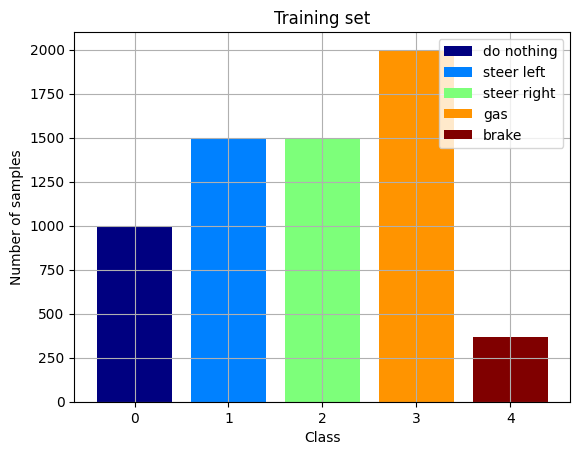
\includegraphics[width=0.4\textwidth]{figures/images/train_set.png}
        \label{fig:train_set}
    }
    \subfloat[Validation set.]{
        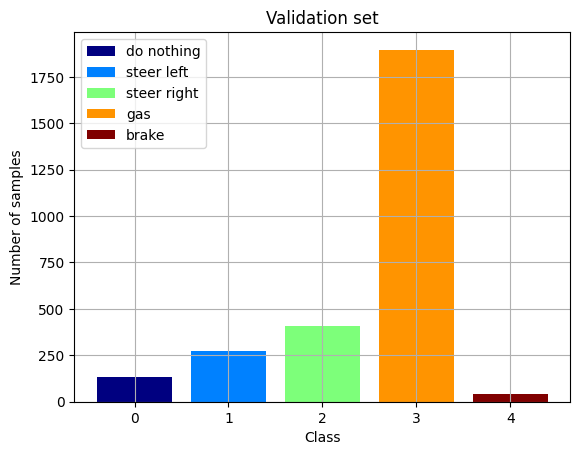
\includegraphics[width=0.4\textwidth]{figures/images/test_set.png}
        \label{fig:test_set}
    }
    \caption{Composition of the dataset.}
\end{figure}

\noindent \\Another aspect to consider is the information contained in a single observation. In fact, it is common practice to preprocess images before feeding them into a classification model (both instances belonging to the dataset and not), mainly to reduce computational load and to improve training performance.
\\For this particular problem, the following manipulations are applied:

\begin{enumerate}
    \item the texture of the grass is made uniform;
    \item the saturation is enhanced;
    \item the colors are converted to grayscale;
    \item the reward counter in the lower left corner is concealed;
    \item the elements of the tensor are normalized to 1.
\end{enumerate}

\noindent This way, we expect the model to converge more easily to an acceptable solution and to have fewer issues in generalizing what it will learn from the data. \\In Fig. \ref{fig:sample_preprocessed} the preprocessing of the previous random sample is carried out as an example.
\begin{figure}[htbp]
    \centering
    \subfloat[A random sample of the dataset.]{
        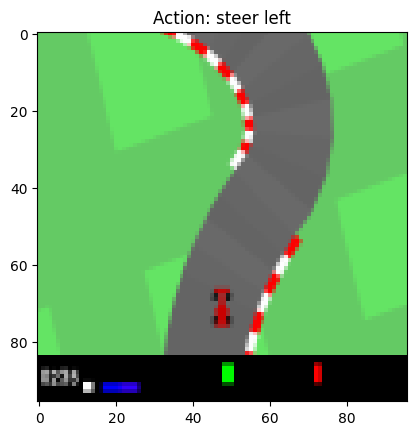
\includegraphics[width=0.35\textwidth]{figures/images/sample.png}
        \label{fig:sample}
    }
    \subfloat[The same sample after preprocessing.]{
        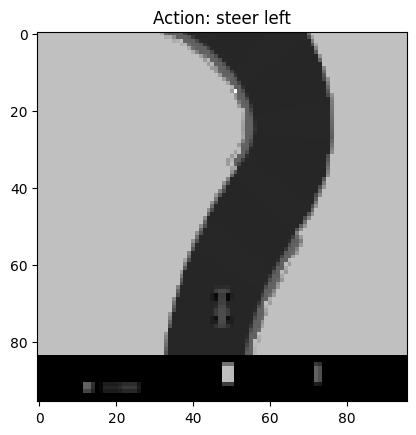
\includegraphics[width=0.35\textwidth]{figures/images/sample_preprocessed.png}
        \label{fig:sample_preprocessed}
    }
    \caption{Effect of preprocessing on the observations.}
\end{figure}
\subsection{CNN tuning and fitting}
\label{sec:cnn_tuning_fitting}

\noindent As requested, two convolutional neural networks have been implemented and trained. 

\noindent \\The idea behind model 0 is to implement large filters that are able to capture the general structure of the input image (i.e., a tensor of shape $96 \times 96 \times 1$), which shrink in size as the network goes deeper. The fully-connected section is composed of three dense layers of decreasing number of units.
\\On the other hand, model 1 implements smaller filters that are able to capture the details of the observations. Its dense part is made of two layers with a greater number of units than model 0.

\noindent \\For both structures, depicted in Fig. \ref{fig:model_structures}, the following choices have been made:

\begin{itemize}
    \item the activation function is ReLU, except for the output layer, where softmax is used to obtain a probability distribution over the 5 classes;
    \item the convolutional layers are followed by a max pooling layer with strides always equal to the pool size in order to reduce the dimensionality of the feature maps;
    \item overfitting is prevented by using dropout layers after the dense layers, and by applying weight decay (with l2 regularization penalty always equal to 0.001) to the convolutional and dense layers.
\end{itemize}

\tikzstyle{input_block} = [rectangle, draw, fill=gray!20, align=center, rounded corners, minimum height=0.6cm, font=\small]
\tikzstyle{conv_block1} = [rectangle, draw, fill=blue!20, text centered, rounded corners, text width=4.5cm, minimum height=0.6cm, font=\small]
\tikzstyle{conv_block2} = [rectangle, draw, fill=blue!20, text centered, rounded corners, text width=3.9cm, minimum height=0.6cm, font=\small]
\tikzstyle{dense_block} = [rectangle, draw, fill=orange!20, text centered, rounded corners, minimum height=0.6cm, font=\small]
\tikzstyle{dropout_block} = [rectangle, draw, fill=red!20, text centered, rounded corners, minimum height=0.6cm, font=\small]
\tikzstyle{activation_block} = [rectangle, draw, fill=green!20, text centered, rounded corners, minimum height=0.6cm, font=\small]
\tikzstyle{pooling_block} = [rectangle, draw, fill=purple!20, text centered, rounded corners, minimum height=0.6cm, font=\small]
\tikzstyle{flatten_block} = [rectangle, draw, fill=yellow!20, text centered, rounded corners, minimum height=0.6cm, font=\small]

\tikzstyle{arrow} = [thick,->,>=stealth]

\begin{figure}[htbp]
    \centering
    \subfloat[Structure of model 0.]{
        \begin{tikzpicture}[node distance=1cm]
            % Input
            \node (input) [input_block] {\textbf{Input}: shape=(96, 96, 1)};
            
            % Conv1
            \node (conv1) [conv_block1, below=0.8cm of input] {\textbf{Conv2D}: filters=8, kernel=7, strides=3, L2 
                penalty=0.001};
            \node (act1) [activation_block, below=0.3cm of conv1] {\textbf{Activation}: ReLU};
            \node (pool1) [pooling_block, below=0.3cm of act1] {\textbf{MaxPooling2D}: pool size=2, strides=2};
            
            % Conv2
            \node (conv2) [conv_block2, below=0.8cm of pool1] {\textbf{Conv2D}: filters=16, kernel=4, L2 penalty=0.001};
            \node (act2) [activation_block, below=0.3cm of conv2] {\textbf{Activation}: ReLU};
            \node (pool2) [pooling_block, below=0.3cm of act2] {\textbf{MaxPooling2D}: pool size=2, strides=2};
            
            % Flatten
            \node (flatten) [flatten_block, below=0.8cm of pool2] {\textbf{Flatten}};
            
            % Dense1
            \node (dense1) [dense_block, below=0.8cm of flatten] {\textbf{Dense}: units=128, L2 penalty=0.001};
            \node (drop1) [dropout_block, below=0.3cm of dense1] {\textbf{Dropout}: rate=0.4};
            \node (act3) [activation_block, below=0.3cm of drop1] {\textbf{Activation}: ReLU};
            
            % Dense2
            \node (dense2) [dense_block, below=0.8cm of act3] {\textbf{Dense}: units=64, L2 penalty=0.001};
            \node (drop2) [dropout_block, below=0.3cm of dense2] {\textbf{Dropout}: rate=0.3};
            \node (act4) [activation_block, below=0.3cm of drop2] {\textbf{Activation}: ReLU};
            
            % Output
            \node (dense3) [dense_block, below=0.8cm of act4] {\textbf{Dense}: units=5};
            \node (act5) [activation_block, below=0.3cm of dense3] {\textbf{Activation}: softmax};
            
            % Arrows
            \draw [arrow] (input) -- node[right] {(96, 96, 1)} (conv1);
            
            \draw [arrow] (conv1) -- (act1);
            \draw [arrow] (act1) -- (pool1);
            \draw [arrow] (pool1) -- node[right] {(15, 15, 8)} (conv2);
            
            \draw [arrow] (conv2) -- (act2);
            \draw [arrow] (act2) -- (pool2);
            \draw [arrow] (pool2) -- node[right] {(6, 6, 16)} (flatten);
            
            \draw [arrow] (flatten) -- node[right] {(576)} (dense1);

            \draw [arrow] (dense1) -- (drop1);
            \draw [arrow] (drop1) -- (act3);
            \draw [arrow] (act3) -- node[right] {(128)} (dense2);
            
            \draw [arrow] (dense2) -- (drop2);
            \draw [arrow] (drop2) -- (act4);
            \draw [arrow] (act4) -- node[right] {(64)} (dense3);
            
            \draw [arrow] (dense3) -- (act5);
            
        \end{tikzpicture}
    }
    \hspace{0.5cm}
    \subfloat[Structure of model 1.]{
        \begin{tikzpicture}[node distance=1cm]
            % Input
            \node (input) [input_block] {\textbf{Input}: shape=(96, 96, 1)};
            
            % Conv1
            \node (conv1) [conv_block1, below=0.8cm of input] {\textbf{Conv2D}: filters=6, kernel=3, strides=2, L2 penalty=0.001};
            \node (act1) [activation_block, below=0.3cm of conv1] {\textbf{Activation}: ReLU};
            \node (pool1) [pooling_block, below=0.3cm of act1] {\textbf{MaxPooling2D}: pool size=3, strides=3};
            
            % Conv2
            \node (conv2) [conv_block2, below=0.8cm of pool1] {\textbf{Conv2D}: filters=12, kernel=5, L2 penalty=0.001};
            \node (act2) [activation_block, below=0.3cm of conv2] {\textbf{Activation}: ReLU};
            \node (pool2) [pooling_block, below=0.3cm of act2] {\textbf{MaxPooling2D}: pool size=2, strides=2};
            
            % Flatten
            \node (flatten) [flatten_block, below=0.8cm of pool2] {\textbf{Flatten}};
            
            % Dense1
            \node (dense1) [dense_block, below=0.8cm of flatten] {\textbf{Dense}: units=256, L2 penalty=0.001};
            \node (drop1) [dropout_block, below=0.3cm of dense1] {\textbf{Dropout}: rate=0.4};
            \node (act3) [activation_block, below=0.3cm of drop1] {\textbf{Activation}: ReLU};
            
            % Dense2
            \node (dense2) [dense_block, below=0.8cm of act3] {\textbf{Dense}: units=5};
            \node (act4) [activation_block, below=0.3cm of dense2] {\textbf{Activation}: softmax};
            
            % Arrows
            \draw [arrow] (input) -- node[right] {(96, 96, 1)} (conv1);
            
            \draw [arrow] (conv1) -- (act1);
            \draw [arrow] (act1) -- (pool1);
            \draw [arrow] (pool1) -- node[right] {(15, 15, 6)} (conv2);

            \draw [arrow] (conv2) -- (act2);
            \draw [arrow] (act2) -- (pool2);
            \draw (pool2) -- node[right] {(5, 5, 12)} (flatten);
            
            \draw [arrow] (flatten) -- node[right] {(300)} (dense1);

            \draw [arrow] (dense1) -- (drop1);
            \draw [arrow] (drop1) -- (act3);
            \draw [arrow] (act3) -- node[right] {(256)} (dense2);

            \draw [arrow] (dense2) -- (act4);
        \end{tikzpicture}
    }
    \caption{Comparison of CNN structures. The padding is always \textit{valid}, and where not specified the strides are set to 1.}
    \label{fig:model_structures}
\end{figure}


\noindent Model 0 has 84,901 trainable parameters, while model 1 has 80,213.

\noindent \\About the training phase, take note the following:

\begin{itemize}
    \item in both cases, the maximum epoch number is 50, the batch size is 64, and the loss function is sparse categorical crossentropy (since the labels are integers);
    \item once again to prevent overfitting, early stopping is activated from the 20th epoch onwards with a patience of 6 epochs by monitoring loss over the validation set;
    \item model 0 is trained with the Adam optimizer, while model 1 is trained with Nadam (a variant of Adam that incorporates Nesterov momentum), both with a learning rate of 0.001;
\end{itemize}
\subsection{Model evaluation}
The performance of the two models can be evaluated by looking at some specific metrics. In particular, the following ones are considered:
\begin{enumerate}
    \item \textbf{Loss and accuracy vs. epochs graphs}: observing the trend of these metric during the fitting phase is useful to understand whether the model is overfitting or not;
    \item \textbf{Classification report}: having a look at the main classification metrics both globally and class-wise is particularly useful when the dataset is unbalanced, as in this case;
    \item \textbf{Confusion matrix}: this completes the classification report by showing the number of correct and incorrect predictions for each class.
\end{enumerate}
Obviously, the models could also be evaluated on the basis of how well they manage to drive the car in the Car Racing environment, but since we do not know the ground truth for the actions to be taken in each state or the relation with the validation set, this is not a reliable metric.
\subsection{Hyperparameter fine-tuning}
After the the training and evaluation phases are over, we may consider how satisfactory the results are and whether we can improve them by tuning the hyperparameters. There are lots of hyperparameters that can be fine-tuned, and as a matter of fact the ones in the models described in Sec. \ref{sec:cnn_tuning_fitting} and shown in Fig. \ref{fig:model_structures} are not chosen randomly, but they are the result of a preliminary tuning phase based on trial and error that is not reported here for the sake of brevity.
\\Instead, we are only going to focus on the analysis of the hyperparameters whose effect is more evident (see Sec. \ref{sec:effect_of_class_weights}), namely the weights of the classes used during training, by relating them to the aforementioned performance metrics.

\section{Results}
\begin{figure}[htbp]
    \centering
    \subfloat[Model 0.]{
        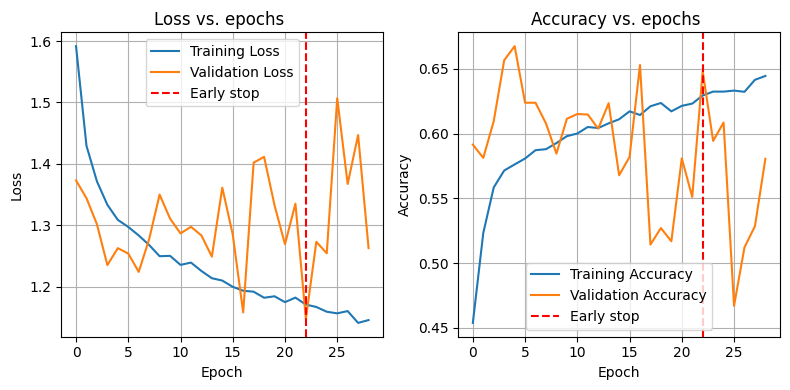
\includegraphics[width=0.7\textwidth]{figures/images/epochs_m0.png}
        \label{fig:epochs_m0}
    }
    \\
    \subfloat[Model 1.]{
        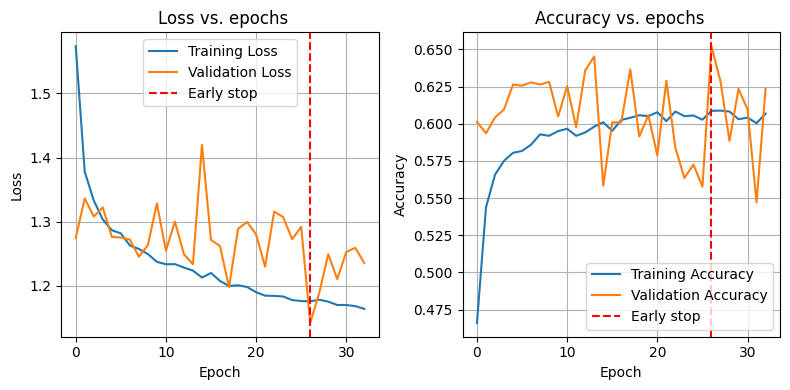
\includegraphics[width=0.7\textwidth]{figures/images/epochs_m1.png}
        \label{fig:epochs_m1}
    }
    \caption{Graph of loss and accuracy of the two models during the training phase, highlighting the point of early stopping.}
    \label{fig:epochs}
\end{figure}
\subsection{Classification scores}
\label{sec:classification_scores}
Even though we have taken many precautions with the purpose of maximizing the performance of the models, the actual results turned out to be quite disappointing. As a matter of fact, the classification reports in Tab. \ref{tab:report} show that the models are not able to correctly classify a great portion of the samples in the validation set.
\\The important thing to notice is that the lowest scores come from the classification of class 4, i.e. \textit{brake}. The reason for this is probably due to the fact that it is the least represented in the dataset, and therefore the models have not been able to learn the features that characterize them. This is confirmed by the fact that the results become proportionally better the higher the number of samples in the specific class, even though they are still far from being good.

\begin{table}[htbp]
    \centering
    
    \begin{subtable}{\textwidth}
        \centering
        \begin{tabular}{cccc}
            \toprule
            \textbf{Class} & \textbf{Precision} & \textbf{Recall} & \textbf{F1-score} \\
            \midrule
            0 & 0.24 & 0.47 & 0.31 \\
            1 & 0.38 & 0.58 & 0.46 \\
            2 & 0.52 & 0.68 & 0.59 \\
            3 & 0.87 & 0.68 & 0.76 \\
            4 & 0.05 & 0.08 & 0.06 \\
            \midrule
            \textbf{Accuracy} & & & 0.65 \\
            \textbf{Macro avg} & 0.41 & 0.50 & 0.44 \\
            \textbf{Weighted avg} & 0.72 & 0.65 & 0.67 \\
            \bottomrule
        \end{tabular}
        \caption{Model 0.}
    \end{subtable}
    \vspace{0cm}\\

    \begin{subtable}{\textwidth}
        \centering
        \begin{tabular}{cccc}
            \toprule
            \textbf{Class} & \textbf{Precision} & \textbf{Recall} & \textbf{F1-score} \\
            \midrule
            0 & 0.28 & 0.38 & 0.32 \\
            1 & 0.36 & 0.54 & 0.43 \\
            2 & 0.49 & 0.65 & 0.56 \\
            3 & 0.84 & 0.70 & 0.77 \\
            4 & 0.06 & 0.05 & 0.05 \\
            \midrule
            \textbf{Accuracy} & & & 0.65 \\
            \textbf{Macro Avg} & 0.40 & 0.46 & 0.43 \\
            \textbf{Weighted Avg} & 0.70 & 0.65 & 0.67 \\
            \bottomrule
        \end{tabular}
        \caption{Model 1.}
    \end{subtable}
    
    \caption{Classification reports of the two models, showing class-wise precision, recall and f1-score, and global accuracy over the validation set.}
    \label{tab:report}
\end{table}

\noindent The increased level of detail provided by confusion matrices (see Fig. \ref{fig:conf_mat}) does not tell a different story. However, it is way more useful when it comes to adjusting the models in order to make them drive in the Car Racing environment: for instance, steering left instead of braking on a straight is not as big of a deal as accelerating instead of braking when a curve is coming up.

\begin{figure}[htbp]
    \centering
    
    \subfloat[Model 0.]{
        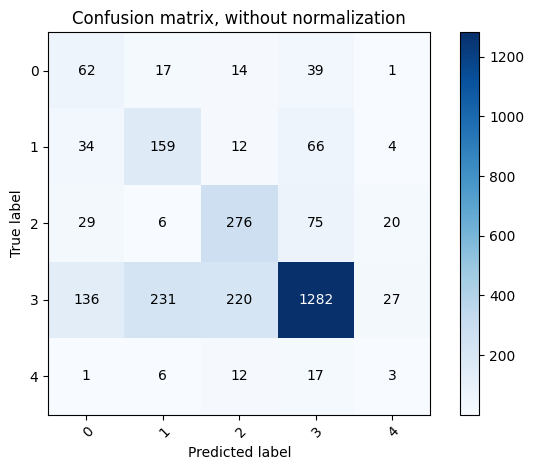
\includegraphics[width=0.4\textwidth]{figures/images/conf_mat_m0.png}
        \label{fig:conf_mat_m0}
    }
    \subfloat[Model 1.]{
        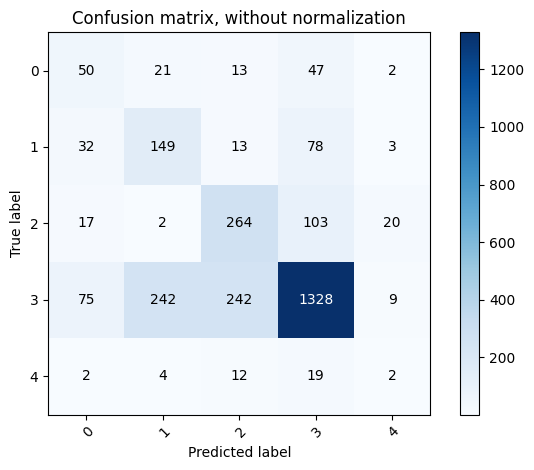
\includegraphics[width=0.4\textwidth]{figures/images/conf_mat_m1.png}
        \label{fig:conf_mat_m1}
    }

    \caption{Confusion matrices of the two models over the validation set.}
    \label{fig:conf_mat}
\end{figure}

\noindent \\After having tried with minimum improvement and considerable effort to obtain better performance by tuning the structures and the hyperparameters of the models (see Sec. \ref{sec:effect_of_class_weights}), the logical conclusion is that the dataset needs to be improved and possibly its split into training and validation sets needs to be changed and/or randomized.




\subsection{Effect of class weights}
\label{sec:effect_of_class_weights}
In the previous section we have speculated that the poor performance of the CNN on the test set is due to the unbalanced nature of the dataset. Among the most common techniques to deal with unbalanced datasets, using class weights is one of the simplest and most effective (unlike oversampling, it does not require additional computing power, nor does it cause loss of information in the dataset like undersampling). In this section we will evaluate the effect of different class weights on the validation performance of the CNNs.
\\ The experiments were carried out with the configurations transcribed in Tab. \ref{tab:class_weights}. In particular, observe that:
\begin{itemize}
    \item \textbf{W1} corresponds to the default configuration, i.e. no class weights;
    \item \textbf{W2} is computed automatically to balance the training set;
    \item \textbf{W3} is composed of the ratios between the number of samples in each class in the test set and in the training set;
    \item the remainder is chosen arbitrarily.
\end{itemize}

\begin{table}[ht]
    \centering
        \begin{tabular}{cccccc}
        \hline
        \textbf{Weights} & \textbf{Class 0} & \textbf{Class 1} & \textbf{Class 2} & \textbf{Class 3} & \textbf{Class 4} \\ \hline
        W1                     & 1.000            & 1.000            & 1.000            & 1.000            & 1.000            \\
        W2                     & 1.274            & 0.849            & 0.849            & 0.637            & 3.452            \\
        W3                     & 0.133            & 0.183            & 0.271            & 0.948            & 0.106            \\
        W4                     & 1.200            & 1.000            & 1.000            & 0.700            & 2.200            \\
        W5                     & 0.900            & 1.000            & 1.000            & 0.800            & 1.800            \\
        W6                     & 1.000            & 1.000            & 1.000            & 0.200            & 2.000            \\
        W7                     & 0.600            & 0.700            & 0.700            & 0.400            & 2.000            \\ \hline
        \end{tabular}
    \caption{Class weights used for the experiments.}
    \label{tab:class_weights}
\end{table}

\noindent As seen in Sec. \ref{sec:classification_scores}, evaluating the class-wise performance is as crucial as evaluating the overall one. For the latter we can use validation loss (do not forget that this is the metric monitored by the early stopping callback, hence we will necessarily look at the best one after epoch 20), while for the former we may use f1-score, which summarizes the precision and recall scores for each class. 

\noindent \\The plots in Fig. \ref{fig:weights_loss} and \ref{fig:weights_f1} show the outcomes of the experiments. Observe that:
\begin{itemize}
    \item using no class weights (W1) is definitely better than using the ones computed automatically (W2), since the validation set unbalance is even more severe than the training set one;
    \item W3 is the best configuration in terms of validation loss since it is taylored on the test set, but it scores 0 in terms of f1-score for class 4 for both models, thus it would not be a good choice for driving the race car;
    \item W6 penalizes excessively the majority class 3 and (as a consequence) the validation loss skyrockets, thus it is the worst configuration;
    \item finally, the two models score significantly different f1-scores with the same weights - especially using W3 and W6 - but the validation losses are very similar.
\end{itemize}

\begin{figure}[htbp]
    \centering
    \subfloat[Model 0.]{
        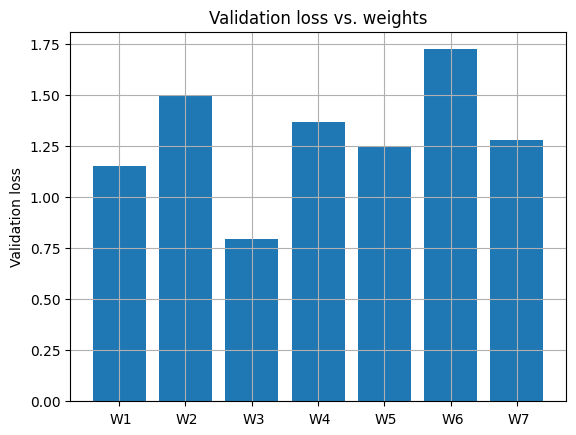
\includegraphics[width=0.4\textwidth]{figures/images/weights_loss_m0.png}
        \label{fig:weights_loss_m0}
    }
    \subfloat[Model 1.]{
        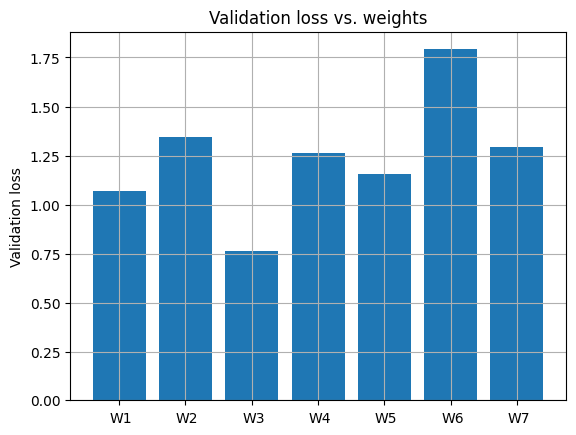
\includegraphics[width=0.4\textwidth]{figures/images/weights_loss_m1.png}
        \label{fig:weights_loss_m1}
    }
    \caption{Effect of different class weights on the validation loss.}
    \label{fig:weights_loss}
\end{figure}
\begin{figure}[htbp]
    \centering
    \subfloat[Model 0.]{
        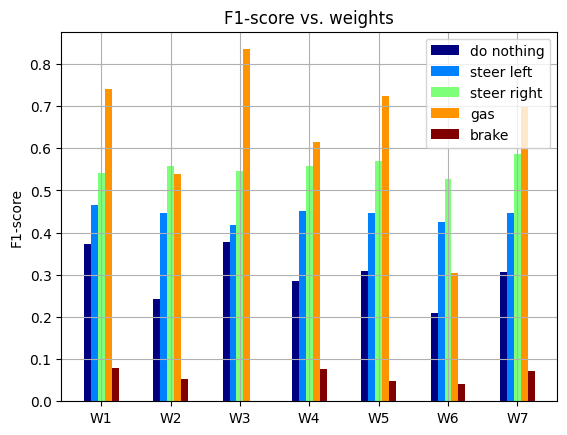
\includegraphics[width=0.4\textwidth]{figures/images/weights_f1_m0.png}
        \label{fig:weights_f1_m0}
    }
    \subfloat[Model 1.]{
        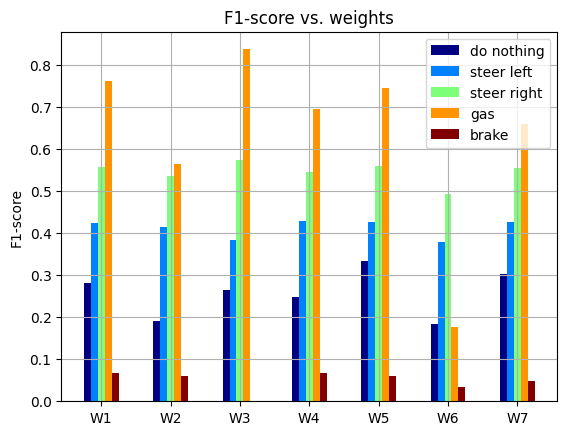
\includegraphics[width=0.4\textwidth]{figures/images/weights_f1_m1.png}
        \label{fig:weights_f1_m1}
    }
    \caption{Effect of different class weights on the class-wise f1-score.}
    \label{fig:weights_f1}
\end{figure}

\noindent The final choice of weights is W4, which is the one that provides the best trade-off between validation loss, f1-scores and driving capabilities (see App. \ref{sec:driving_race_car}). As a matter of fact, the results reported in the previous sections were obtained with this configuration.

\section{Conclusions}
Let us sum up the main results of this report. Two different CNNs (with different structures and hyperparameters) have been built and used to solve the image classification problem that was proposed. The dataset has been preprocessed in order to delete unnecessary and/or misleading information. With the objective of improving performance, adjustments have been made, precautions have been taken and experiments have been carried out. The threat of overfitting has been kept away with regularization strategies and early stopping.
Moreover, the analysis of the performance in realtion to the class weights has shown that the choice of the weights is crucial for the success of the models.

\noindent \\Despite these efforts, though, the final results are not outstanding: the main problem could be that the dataset is not sufficient to train a CNN that can generalize well, especially on the given validation set, which is quite different from the training set. Supporting this there is the fact that the models score quite similarly to each other in the tests that have been conducted, so the problem would not seem to reside in the network tuning phase.

\appendix
\section{Driving a race car}
\label{sec:driving_race_car}
In order to allow the two models to drive a race car in the Car Racing environment, they should be included in a feedback loop, as shown in Figure \ref{fig:game_loop}. Based on an initial observation, the agent (the CNN) takes an action, which is passed to the environment. The environment then computes a response and returns a new observation, which is passed to the agent. The agent then takes another action, and so on, until the game ends (because of the car either crashing or completing a full lap, or because of the expiration of the maximum time of 30 seconds).

\tikzstyle{block} = [rectangle, draw, fill=gray!20, align=center, rounded corners, minimum height=1cm, font=\small]

\begin{figure}[htbp]
    \centering
    \begin{tikzpicture}
        \node [block] (block1) {Agent (CNN)};
        \node [block, right=2cm of block1] (block2) {Environment};
        
        \path[->] (block1) edge [bend left=45] node[above] {Action} (block2);
        \path[->] (block2) edge [bend left=45] node[below] {Observation} (block1);
    \end{tikzpicture}
    \caption{Closed loop between the CNN and the Car Racing environment.}
    \label{fig:game_loop}
\end{figure}


\noindent Mainly due to the class weights choice of Sec. \ref{sec:effect_of_class_weights}, both the models are capable of playing the racing game with a good degree of success on a great number of randomly-generated tracks, as shown in Fig. \ref{fig:car_racing} and in the video linked in the footnote\footnote{YouTube video showing the two models driving on randomly-generated tracks: \url{https://youtu.be/EUGlU5wEMvg}}. However, there is still a lot of room for improvement, as the models sometimes act in a way that is not optimal and that can possibly lead to "crashes", as shown in Fig. \ref{fig:car_racing_fail}. With this in mind, it would probably be best to combine a CNN model with one of reinforcement learning that also exploits the reward system of the Gym environment.

\begin{figure}[htbp]
    \centering
    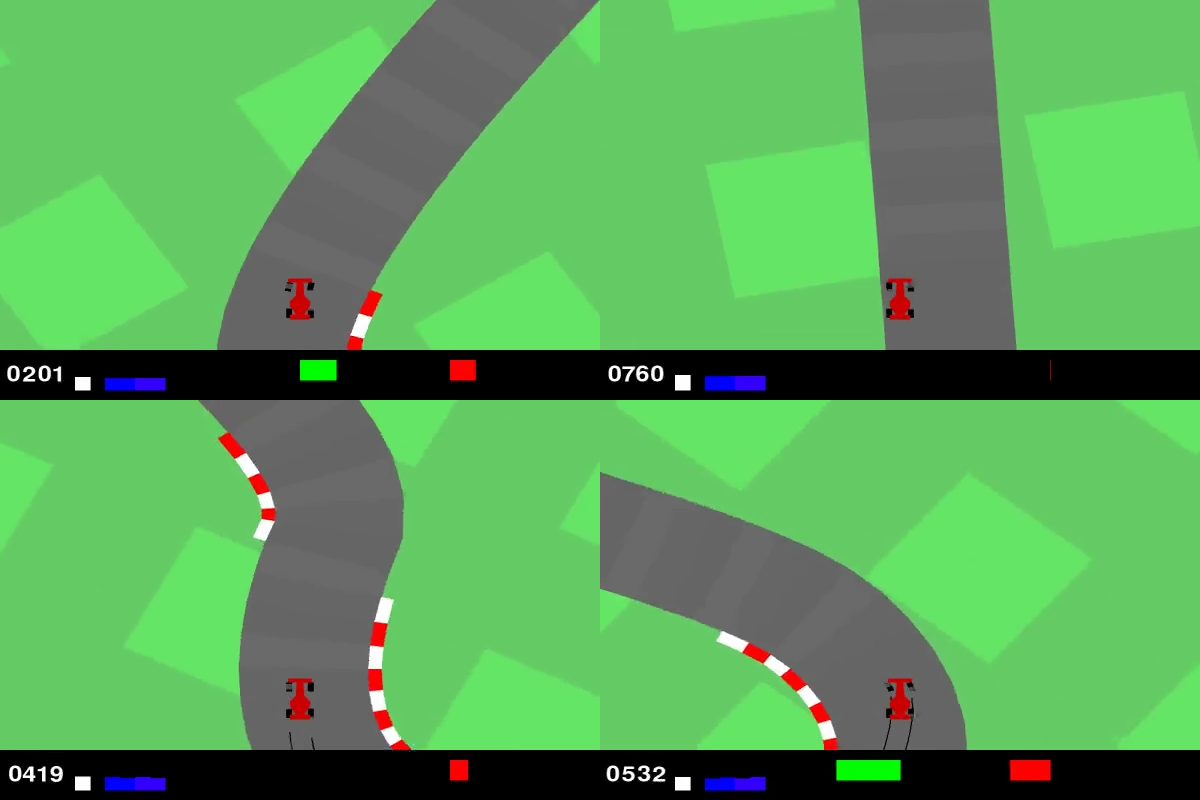
\includegraphics[width=0.75\textwidth]{figures/images/car.png}
    \caption{The models driving in the Car Racing environment.}
    \label{fig:car_racing}
\end{figure}


\begin{figure}[htbp]
    \centering
    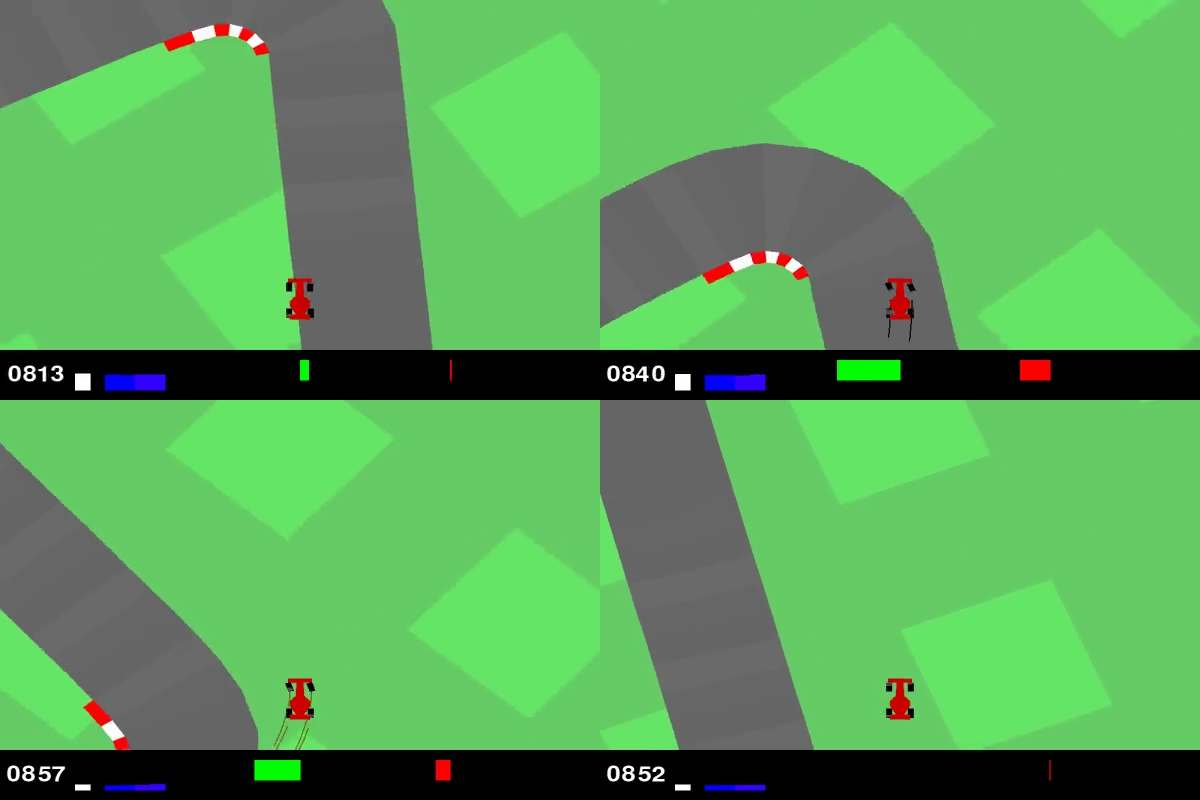
\includegraphics[width=0.75\textwidth]{figures/images/car_fail.png}
    \caption{Model 0 causing the race car to skid off the road.}
    \label{fig:car_racing_fail}
\end{figure}





\end{document}
